\documentclass[11pt, A4 paper, twocolumn ]{article}

% Packages
\usepackage{palatino}
\usepackage{url}
\usepackage{latexsym}
\usepackage{lipsum}
\usepackage{titlesec}
\usepackage{geometry}
\usepackage{amssymb}
\usepackage{mathtools, nccmath}
\usepackage{enumerate}
\usepackage{tikz}   
\usepackage{graphicx}
\usepackage{caption}
\usepackage{subcaption}
\usepackage{float}
\usepackage[superscript,biblabel]{cite}
\usepackage{fancyhdr}
\usepackage{hyperref}

% Customize link appearance
\hypersetup{
	colorlinks=true,
	linkcolor=blue,
	filecolor=magenta,      
	citecolor=red
}

% Tikz for flow charts
\usetikzlibrary{shapes.geometric, arrows}   

% Custom commands
\newcommand{\fc}{$ f_{\text{C}} $}
\newcommand{\fcm}{f_{\text{C}}}
\newcommand{\fr}{$ f_{\text{R}} $}
\newcommand{\frm}{f_{\text{R}}}

% Set page lengths and margins
\setlength{\paperwidth}{21cm}   % A4
\setlength{\paperheight}{29.7cm} % A4
\setlength\topmargin{-0.5cm}    
\setlength\oddsidemargin{-1cm}   
\setlength\textheight{24cm} 
\setlength\textwidth{18.0cm}
\setlength\columnsep{0.8cm}  
\newlength\titlebox 
\setlength\titlebox{5cm}
\setlength\headheight{1pt}   
\setlength\headsep{30pt}

% Page style and headers
\pagestyle{fancy}
\fancyhead[L]{Project Report (PHY 302)}
\fancyhead[R]{Srishti Patil}
\fancypagestyle{firstpage}{%
	\lhead{Project Report (PHY 302)}
	\rhead{IISER-Pune}
}

% Title and author
\title{{\Huge Evolution of Cooperation Among Autonomous Agents in the Presence of Public Information} }
\author{Srishti Patil\\ Supervisor: M.S. Santhanam}
\date{January, 2021}


\begin{document}
	\maketitle
	\thispagestyle{firstpage}
	\section{Introduction}
		\vspace{-0.5cm}
		In games like Prisoner's Dilemma and the Public Goods game, defection is theoretically the dominant strategy. Therefore, it is hard to sustain cooperation \cite{old_repeated, tragedy} in the classical repeated Prisoner's Dilemma game in a well-mixed population. This is often at odds with reality where cooperation is ubiquitous, and thus understanding the emergence and persistence of altruistic behaviour in this setting poses an interesting challenge. Evolutionary Game Theory provides a mathematical framework to explore this problem. Previous work on the topic \cite{gametheoryandphysics, Shirado} has focused on spatial reciprocity \cite{spatial_reciprocity, stratification} and nearest neighbour interactions among agents. The relevant results have been summarized in Figure \ref{fig:imitate}. These are reproduced from the paper by C. Hauert and G. Szab\'{o} \cite{gametheoryandphysics}. \par 
		In other related works, incentivisation such as social rewarding \cite{reward, social_reward, replicator_dynamics, antisocial_rewarding}  and punishment \cite{punishment, synergy, shared_cost, overpunishing}, is seen to be an effective method to promote cooperation. Other mechanisms like memory effect among agents \cite{memory_effect}, incomplete information \cite{incomplete_info}, external forcing \cite{external_forcing} have proven effecitve. The aspect of public information is relatively unexplored and extremely relevant in such systems since the end-goal is to promote collective good. \par 
		The aim of this project is to understand the effect of public information \cite{publicinfo_china} and reputation \cite{inferring_reputation} in finitely repeated spatial games (mainly Prisoner's Dilemma).  In Section \ref{sec:models}, three new models are proposed - \textit{Pdist, fcT } and \textit{Rep}. Results are shown and discussed in Section \ref{sec:results}. Section \ref{sec:opdyn} explores in brief, an application of one of the models on a real-world problem. Further details about the models and results are listed in Appendix~\ref{appendix} \par
	
		% Previous results (replicated from Hauert paper)
		\begin{figure}[h]
		\centering
		\begin{subfigure}[b]{0.23\textwidth}
			\centering
			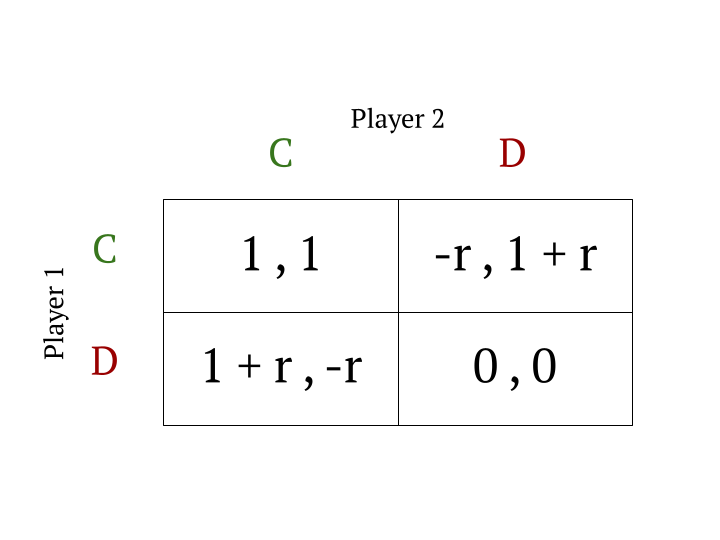
\includegraphics[width=\textwidth]{graphs/payoff-matrix}
			\caption{}
			\label{fig:payoff-matrix}
		\end{subfigure}
		\begin{subfigure}[b]{0.23\textwidth}
			\centering
			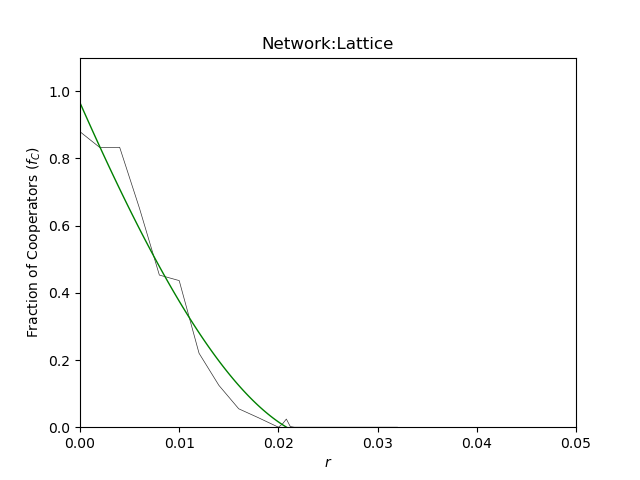
\includegraphics[width=\textwidth]{graphs/lat-imitate}
			\caption{}
			\label{fig:lat-imitate}
		\end{subfigure}
		\begin{subfigure}[b]{0.23\textwidth}
			\centering
			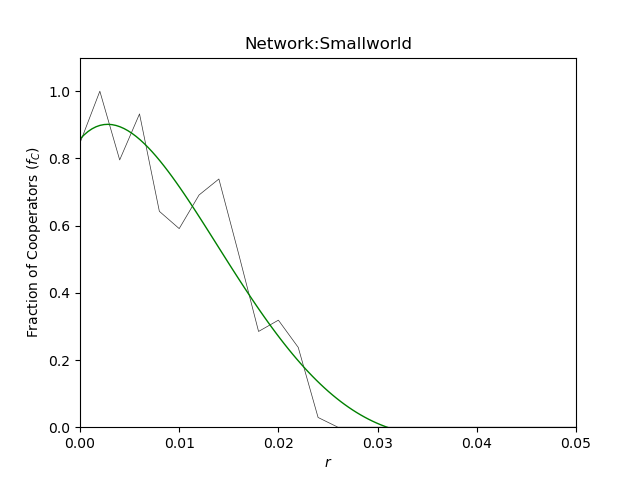
\includegraphics[width=\textwidth]{graphs/sw-imitate}
			\caption{}
			\label{fig:sw-imitate}
		\end{subfigure}
		\begin{subfigure}[b]{0.23\textwidth}
			\centering
			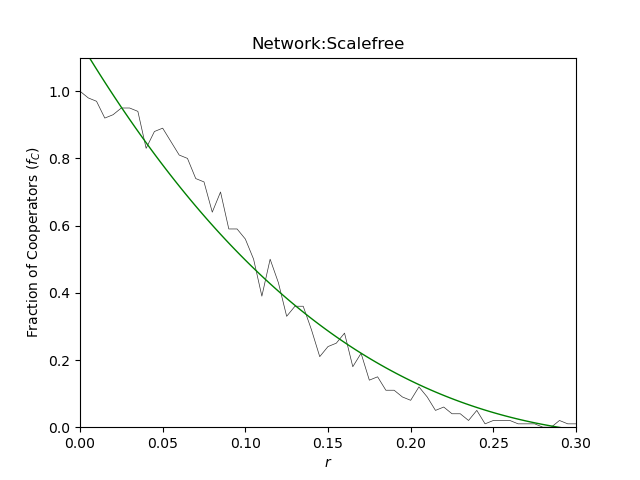
\includegraphics[width=\textwidth]{graphs/sf-imitate}
			\caption{}
			\label{fig:sf-imitate}
		\end{subfigure}
		\caption{\footnotesize \textit{(a)} The payoff matrix for Prisoner's Dilemma Game. $ r $ is the cost to benefit ratio.
		\textit{(b)} $ f_{C} $ vs $ r $ plot for repeated prisoner's dilemma on a regular lattice network. $ f_{C} $ vanishes around $ x \approx 0.02 $
	\textit{(c)} $ f_{C} $ vs $ r $ plot for repeated prisoner's dilemma on a smallworld network. $ f_{C} $ vanishes around $ x \approx 0.03 $
\textit{(d)} $ f_{C} $ vs $ r $ plot for repeated prisoner's dilemma on a scalefree network. $ f_{C} $ vanishes around $ x \approx 0.3 $ }
		\label{fig:imitate}
	\end{figure}
		
	\section{Models} \label{sec:models}
		Three models have been introduces as mechanisms to understand and enhance 	cooperation among agents playing the Prisoner's Dilemma game on different network topologies (Regular Lattice, Scalefree, Small-World). Each node represents an agent and 	each agent has two actions (strategies) - Cooperation and Defection. \par 
		Every iteration (Monte Carlo Step) of the game allows, on an average, one agent (agent $i$) to update its strategy. The rule of updation depends on the model being used. If the agents update their strategies by imitating a randomly chosen nearest neighbour (agent $j$) with a Fermi-Dirac like transition probability function (eq \ref{eq:fermi}) depending on the difference in payoffs (as seen in the existing literature) \cite{review}, 
	
		\begin{equation} \label{eq:fermi}
			W(s_{i} \leftarrow s_{j}) = \frac{1}{1 + \exp[(p_{i} - p_{j})/k]}
		\end{equation}

	 	we get the results shown in Figure \ref{fig:imitate} (replicated results from \cite{gametheoryandphysics}). $p_{i}$ is the payoff of agent $i$ in the current round and $k$ is the noise parameter (here, taken to be $ 0.1 $).  It can be observed that cooperation in the system dies out for low values of parameter $r$ (ratio of cost to benefit of cooperation). 
	
		\subsection{Probability Distribution Model (PDist)} 
			Instead of assigning strategies to agents at the start of the game, we assign for each agent, a probability of adoption to each strategy. At each time step (MCS) all agents update this probability distribution (one by one). \par 
			For agent $i$, the probabiliity of adopting strategy $s$ at time step $t$ ($P_{t}^{s}(i)$) is 	given by equation \ref{eq:pdist}, where $s$ is the strategy that was adopted in the previous timestep. $ \Delta P $ can take a range of values, both positive and negative (see \ref{app:1}) 
			
			\begin{equation}\label{eq:pdist}
				\begin{split}
					&P_{t}^{s}(i) = P_{t-1}^{s}(i) + \Delta P 	\\
					&P_{t}^{-s}(i) = P_{t}^{s}(i) \\
				\end{split}
			\end{equation}

			In this model, the focal agent increases the probability of adoption of the curent strategy ($ s $)  if the payoff is greater than the average payoff in the agent's local neighbourhood. 
	
 	\subsection{fc-Threshold Model (fcT)}
 	To introduce public information to the system, we consider $ f_{\text{C}} $ - the fraction of cooperators in the population. If this information is available to the focal agent (this event occurs with probability $ P_{f_{C}}$), then the updated probability distribution depends on the difference between \fc{} and the focal agent's personal $ \text{threshold}_{\fcm} $ ($ \in [0,1] $). 
 	
 	\begin{equation}\label{fcth-info}
 		\begin{split}
 				&P_{t}^{C} = P_{t-1}^{C}(2-P_{t-1}^{C})^{a} \\
 				&P_{t}^{D} = 1 - P_{t}^{C}
 		\end{split}
 	\end{equation}
 
 where $ a  = (\fcm - \text{threshold}_{\fcm})$ if $\fcm > \text{threshold}_{\fcm}$  and $ 0 $ otherwise. \par 
 If the focal agent does not have access to \fc, then the current strategy ($ s $) is updated according to equation \ref{eq:fcth}. $ a' $ depends on $ p_{i} - p_{\text{avg}} $ (see \ref{app:2} for more details). 
 
 \begin{equation} \label{eq:fcth}
 	\begin{split}
 		&P_{t}^{s} = P_{t-1}^{s}(2-P_{t-1}^{s})^{a'} \\
 		&P_{t}^{-s} = 1 - P_{t}^{s}
 	\end{split}
 \end{equation}

Here, the parameter $ P_{\fcm} $ is a measure of the availablility of public information and the parameter $ \text{threshold}_{\fcm} $ (which is a randomly chosen value between [0,1]) indicates the "tendency" of the agent to use that information. This structure tries to model external influence and personal biases separately. The availibility of external information promotes cooperation as the knowledge of \fc{} gives an indication of how safe it is to cooperate, given that defection is the dominant strategy and cooperation is the risky one from a rational agent's perspective. 

	\subsection{Reputation Model (Rep)}
	This model introduces reputation as a social reward mechanism. Every agent has a reputation value ($ \in  [0,1]$) that increases every time the agent chooses to cooperate (see \ref{app:3}). At each timestep, the focal agent (randomly chosen) will imitate a nearest neighbour based on either the difference in payoffs (the original imitaiton model) or the difference in reputations. The parameter $ p $ decides the probability of choosing imitation based on reputations. \par 
	Public information is in the form of \fr{} - the fraction of population with a reputation above $ 0.9 $. All agents have access to this information. Similar to the \textit{fcT} model, each agent has a "tendency" to use the information denoted by $ \text{threshold}_{\frm} $. If \fr{} is grerater than this personal threshold, then the transition probabililty can be given by equation \ref{eq:rep1}.
	
	\begin{equation} \label{eq:rep1}
		\begin{split}
			&P_{t}^{C} = 	\frac{1}{1 + \exp[-\text{reputation}_{\textit{self}}/k_{r_{1}}]} \\
			&P_{t}^{D} = 1- P_{t}^{C}
		\end{split}
	\end{equation}

	If \fr{} is less than the personal threshold, then the agent resorts to local neighbourhood information (see Figure \ref{flow:rep}). It will pick the agent with maximum reputation  and imitate its strategy with transition probability (eq \ref{eq:rep2}).
	
	\begin{equation}\label{eq:rep2}
		W(s_{i} \leftarrow s_{j}) = \frac{1}{1 + \exp[\text{difference}/k_{r_{2}}]}
	\end{equation}
	\begin{equation*}
	\text{difference} = \text{reputation}_{\textit{self}} - \text{reputation}_{\textit{max}}
	\end{equation*}

	Therefore, if the maximum reputation ($ \text{reputation}_{\textit{max}} $) in the focal agent's neighbourhood is greater than the focal's reputation ($ \text{reputation}_{\textit{self}} $) then the probability of imitating that agent is high. Since reputation is an indication of how much an agent has cooperated in the past, it makes sense to "trust" that agent and imitate its strategy ($ s_{j} $). 
	
	% Flowchart for rep
	\begin{figure}
		\tikzstyle{line} = [draw, -latex']  
		\tikzstyle{cloud} = [draw, text centered, rectangle,node distance=2.5cm, minimum height=1em]  
		\begin{tikzpicture}[node distance = 1cm, auto] % the command node distance is important as it determines the space or the length of the arrow between different blocks.  
			% the command given below are the place of nodes  
			\tikzstyle{every node}=[font=\tiny]
			\node [cloud] (init) {Focal agent chosen at random};  
			\node [cloud, below left of = init, text width=7em](C){Payoff-based Imitation};  
			\node [cloud, below right of = init, text width=7em](D){Reputation-based Imitation};  
			\path[line] (init) -- node[anchor=east] {\textit{1-p}}(C);
			\path[line](init) -- node[anchor=west] {\textit{p}} (D);
			\node[cloud, below of= C, text width=6em,xshift=-1.2cm, yshift=1.2cm](E){Imitate a randomly chosen neighbour based on difference in payoffs};
			\path[line](C) -- (E);
			\node[cloud, below of= D, text width=9em, xshift=-1.2cm] (rep1) {Coordinate with a transition probability that depends on $ \text{reputation}_{\textit{self}} $};
			\path[line](D) -- node[anchor=east] {\fr  $\geq \text{threshold}_{\frm}$} (rep1);
			\node[cloud, below right of=rep1, text width=10em, yshift=0.5cm, xshift=0.5cm] (rep2) {Imitate the neighbour with maximum reputation with a probability that depends on the difference in reputations};
			\path[line]([xshift=7cm]D) -- node[anchor=west] {\fr  $< \text{threshold}_{\frm}$} (rep2);
		\end{tikzpicture} 
	\caption{\small Flowchart for model \textit{Rep}}
	\label{flow:rep}
	\end{figure}

	\section{Results} \label{sec:results}
	All three models \textit{(PDist, fcT and Rep)} enhance cooperation among agents. Figure \ref{fig:results} summarises the results for all the models discussed in the last section. We vary the parameter $ r $ across a range and observe if cooperative behaviour persists. \par 
	
	For model \textit{PDist} (\ref{fig:lat-pdist}, \ref{fig:sw-pdist} and \ref{fig:sf-pdist}), we can see that a low fraction of cooperators survives for even large values of $ r $. For values of parameter $ \Delta P_{\text{max}} $  greater than 0.05, \fc{} vanishes at low $ r $. For scalefree networks, a higher fraction survives. A possible reason for higher values of \fc{} at lower values of   $ \Delta P_{\text{max}} $ may be that for small increments or decrements in the probability distribution allow the system to reach an equilibrium. \par 
	
	Model \textit{fcT} (\ref{fig:lat-fct}, \ref{fig:sw-fct}, \ref{fig:sf-fct}) shows a drastic increase in the equilibrium value of \fc. For values of parameter $ P_{\fcm} > 0.7$, \fc{} is very close to 1 and stays that way for high values of $ r $. To see the effect of public information, we can compare the blue curves ($ P_{\fcm} = 0$) with the rest.  \par 
	
	Results for model \textit{Rep} show that increase in probability of choosing reputation-based imitaiton ($ p $) leads to an increase in \fc. \ref{fig:lat-rep}, \ref{fig:sw-rep} and \ref{fig:sf-rep} do not have any factor of public information. On choosing reputation-based imitation, the focal agent simply looks at its nearest neighbours. \ref{fig:lat-fr}, \ref{fig:sw-fr} and \ref{fig:sf-fr} show the effect of public information for a fixed value of $ p = 0.3$.\par 
	The last row in Figure \ref{fig:results} shows how reputation of all the agents evolves with time. For $ p = 0 $, the values are spread out and have a lower average. For higher values of $ p $, all the agents reach a reputation very close to 1. 
	In general, we observe that introduction of a reward mechanism (reputation) and public information (in models \textit{fcT }and \textit{Rep}) promotes cooperation among agents.
	
		% Results
		\begin{figure*}[p]
		\centering
		\vspace{-0.9cm}
		\begin{subfigure}[b]{0.3\textwidth}
			\centering
			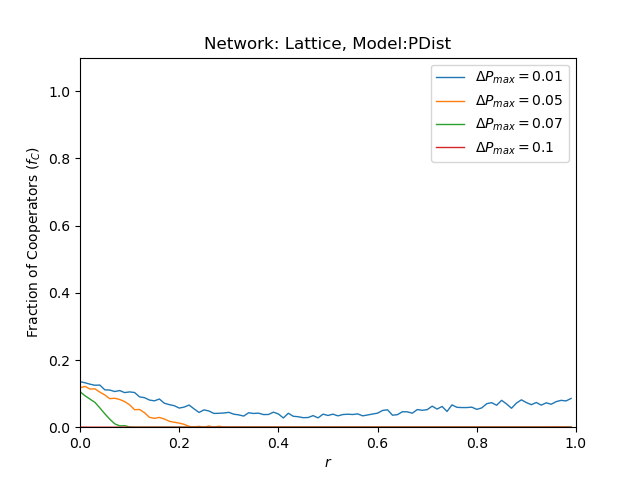
\includegraphics[width=\textwidth]{graphs/lat-pdist}
			\caption{}
			\label{fig:lat-pdist}
		\end{subfigure}
		\begin{subfigure}[b]{0.3\textwidth}
			\centering
			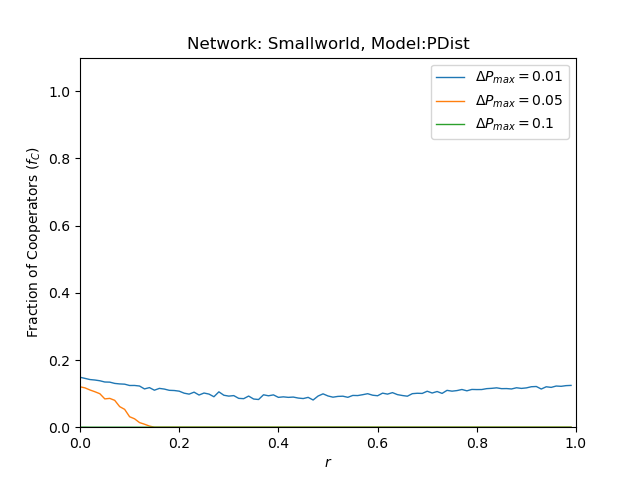
\includegraphics[width=\textwidth]{graphs/sw-pdist}
			\caption{}
			\label{fig:sw-pdist}
		\end{subfigure}
		\begin{subfigure}[b]{0.3\textwidth}
			\centering
			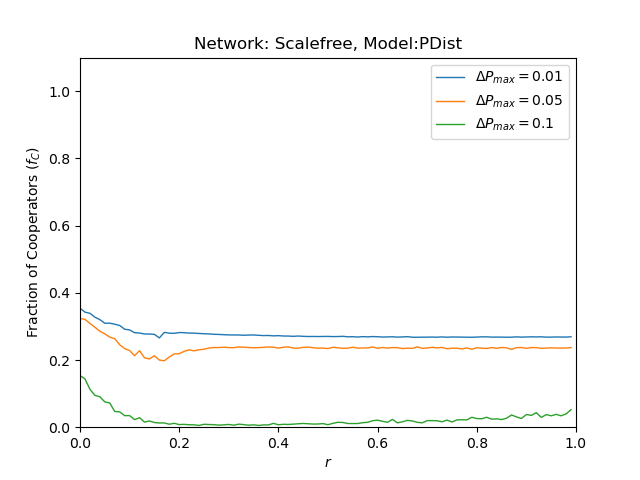
\includegraphics[width=\textwidth]{graphs/sf-pdist}
			\caption{}
			\label{fig:sf-pdist}
		\end{subfigure}
	\begin{subfigure}[b]{0.3\textwidth}
		\centering
		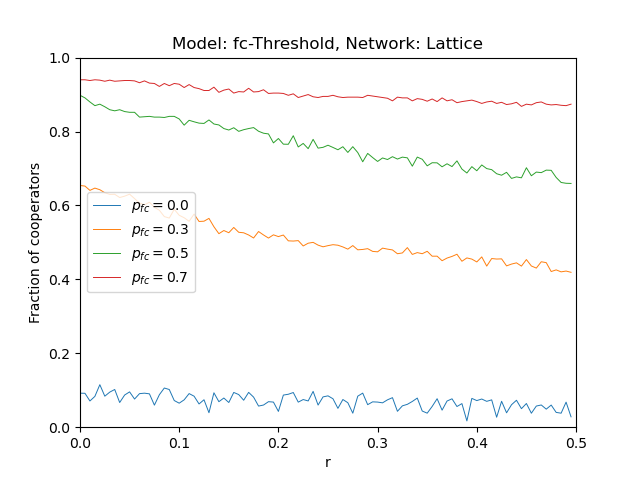
\includegraphics[width=\textwidth]{graphs/varying-pfc-latb2}
		\caption{}
		\label{fig:lat-fct}
	\end{subfigure}
	\begin{subfigure}[b]{0.3\textwidth}
		\centering
		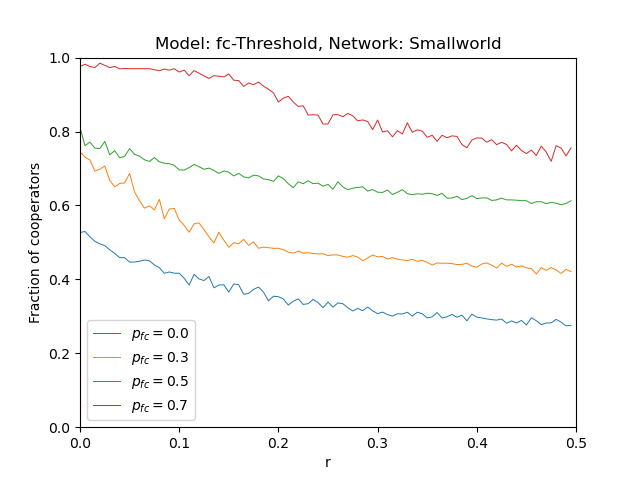
\includegraphics[width=\textwidth]{graphs/varying-pfc-swb2}
		\caption{}
		\label{fig:sw-fct}
	\end{subfigure}
	\begin{subfigure}[b]{0.3\textwidth}
		\centering
		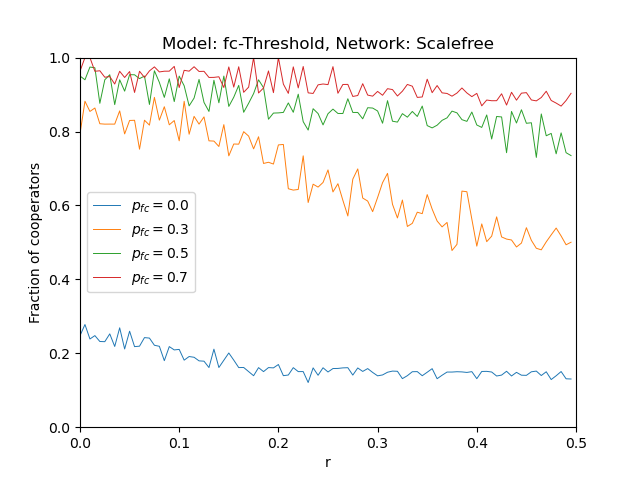
\includegraphics[width=\textwidth]{graphs/varying-pfc-sfb2}
		\caption{}
		\label{fig:sf-fct}
	\end{subfigure}
\begin{subfigure}[b]{0.3\textwidth}
	\centering
	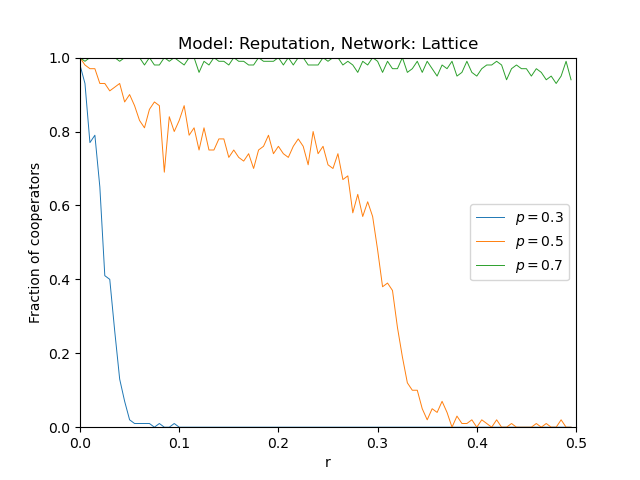
\includegraphics[width=\textwidth]{graphs/fc_r_varyingp_lattice}
	\caption{}
	\label{fig:lat-rep}
\end{subfigure}
\begin{subfigure}[b]{0.3\textwidth}
	\centering
	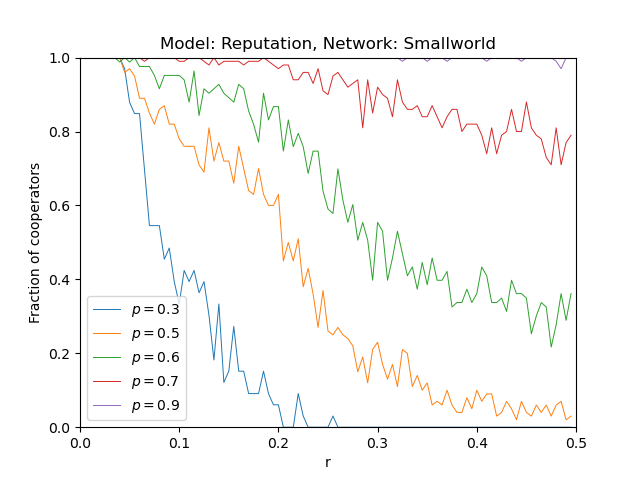
\includegraphics[width=\textwidth]{graphs/fc_r_varyingp_smallworld}
	\caption{}
	\label{fig:sw-rep}
\end{subfigure}
\begin{subfigure}[b]{0.3\textwidth}
	\centering
	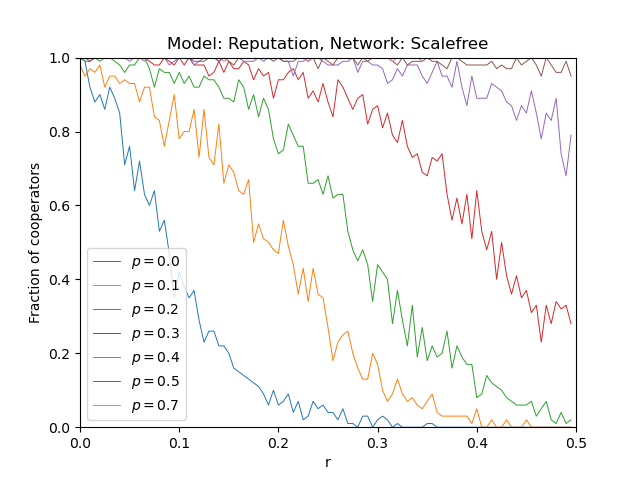
\includegraphics[width=\textwidth]{graphs/fc_r_varyingp_scalefree}
	\caption{}
	\label{fig:sf-rep}
\end{subfigure}
\begin{subfigure}[b]{0.3\textwidth}
	\centering
	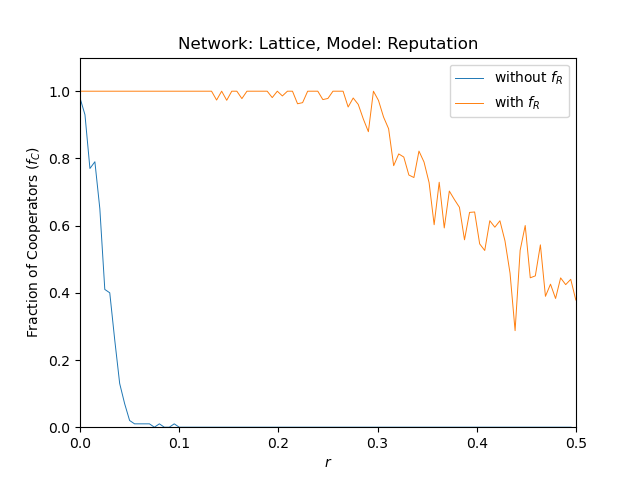
\includegraphics[width=\textwidth]{graphs/lat-fr}
	\caption{}
	\label{fig:lat-fr}
\end{subfigure}
\begin{subfigure}[b]{0.3\textwidth}
	\centering
	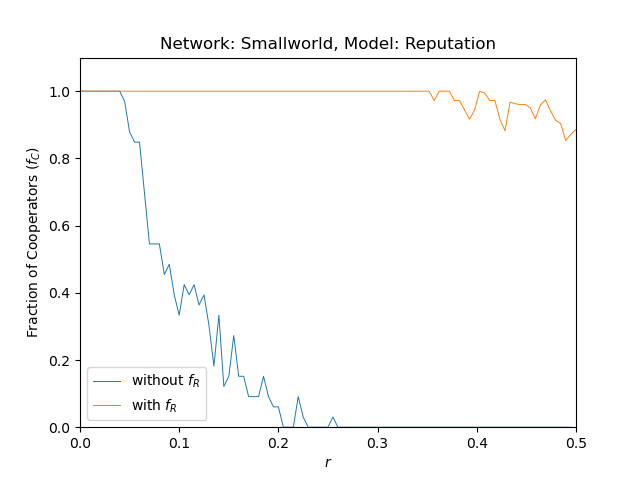
\includegraphics[width=\textwidth]{graphs/sw-fr}
	\caption{}
	\label{fig:sw-fr}
\end{subfigure}
\begin{subfigure}[b]{0.3\textwidth}
	\centering
	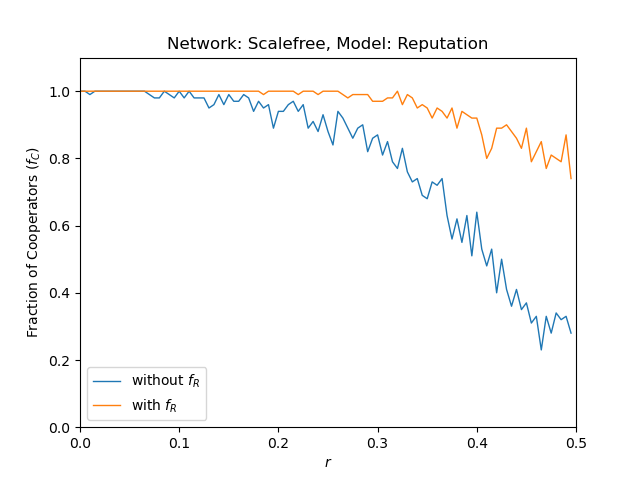
\includegraphics[width=\textwidth]{graphs/sf-fr}
	\caption{}
	\label{fig:sf-fr}
\end{subfigure}
\begin{subfigure}[b]{0.3\textwidth}
	\centering
	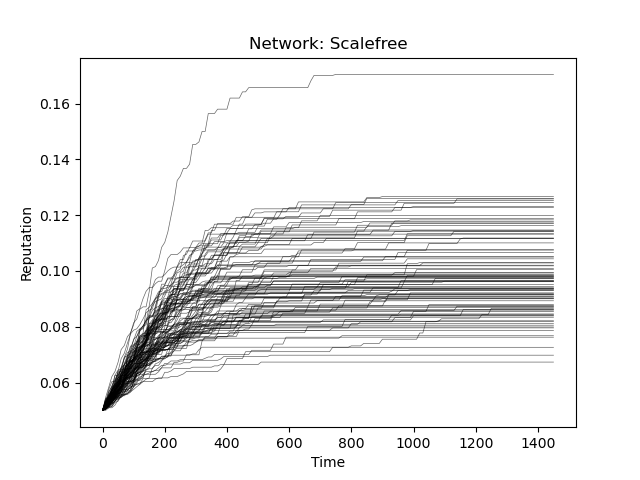
\includegraphics[width=\textwidth]{graphs/rep_te_sfp0.0}
	\caption{}
	\label{fig:repevol1}
\end{subfigure}
\begin{subfigure}[b]{0.3\textwidth}
	\centering
	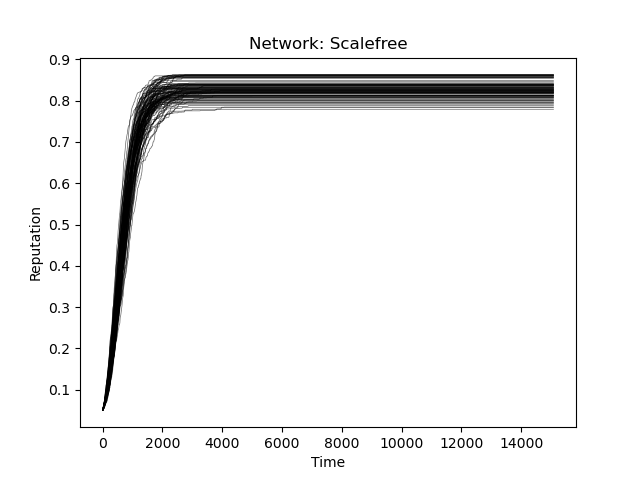
\includegraphics[width=\textwidth]{graphs/rep_te_sfp0.3}
	\caption{}
	\label{fig:repevol2}
\end{subfigure}
\begin{subfigure}[b]{0.3\textwidth}
	\centering
	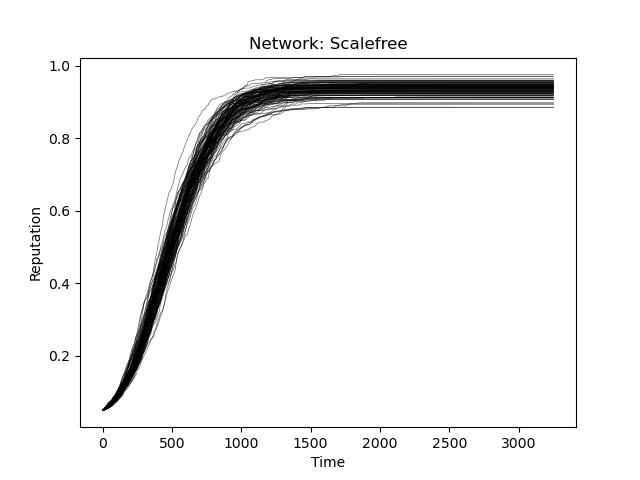
\includegraphics[width=\textwidth]{graphs/rep_te_sfp0.5}
	\caption{}
	\label{fig:repevol3}
\end{subfigure}
		\caption{\footnotesize Row 1: Model \textit{PDist},
			Row 2: Model \textit{fcT}, 
			Row 3: Model \textit{Rep} (varying parameter $ p $),
		Row 4:  Model \textit{Rep} (effect of public information \fr),
	Row 5: Evolution of agent reputations with time (for scalefree network). All plots are generated by averaging over 100 runs on a population size of 100 agents. For smallworld networks, $ Q=0.6 $. Note that due to technological and time constraints, \ref{fig:lat-fr} and \ref{fig:sw-fr} have been run 10 and 35 times respectively.}
		\label{fig:results}
	\end{figure*}
	
	\section{Application in Opinion Dynamics} \label{sec:opdyn}
	Social dilemma games like Prisoner's Dilemma and Public Goods game are inherently asymmetric in that one of the possible strategies is clearly more benefecial for the collective good. In opinion dynamics models (using EGT), the strategies (opinions) have an equal footing. By modifying the \textit{Rep} model, we try to model the effect of public information and reputation on populations of agents that can choose between two opinions (A and B). \par 
	A randomly chosen focal agent, in each timestep, will imitate a nearest neighbour either based on the difference in payoffs or depending on the parameter $ x $ (eq \ref{eq:x}). Imitation based on payoffs should promote the formation of clusters of agents with the same strategy (similar to what we see in \cite{gametheoryandphysics}). Reputation increases in magnitude if an agent adopts the same strategy (sticks to it). It is a reward mechanism that favours one strategy over the other depending on the history of the focal agent. Reputation values range from $ -1 $ to $ 1 $. Negative values correspond to strategy B and positive to startegy A. See appendix \ref{app:4} for details about the transition function and how it depends on $ x $. $ s $ and $ o $ are the reputations of the focal agent and the agent chosen for imitation respectively.  \par 
	
	\begin{equation}\label{eq:x}
		x = \text{sign}(s.o)\left| \frac{o}{s} \right|
	\end{equation}	

 Public information in this model is the fraction of agents with reputation above $0.9 $ (case I - $f_{R}(A) $) or below $ -0.9 $ (case II - $ f_{R}(B) $).To observe the effect of public information, we introduce a new parameter  $ P_{A} $ which is the probability of agents having access to $ f_{R}(A)$. Agents who do not have access to it have access to $ f_{R}(B) $ (see Figure \ref{flow:opdyn}). This parameter is a loose indicator of how well an opinion has been advertised to the masses i.e. the "popularity" of a strategy in the population. We vary this parameter to see how knowing about a strategy's popularity in the population affects the fraction of agents that adopt it in equilibrium. \par 
 Once the focal agent has access to this information, it will adopt the next strategy based on its personal threshold (similar to the one in model \textit{Rep}, see \ref{app:4}) and the sign of its reputation (startegy A if positive, B if negative). The higher the personal threshold, the higher is the probability of adopting the strategy. \par 
 The results for simulations on a regular lattice and a scalefree network are given in Figure \ref{fig:opdyn}. The flat orange line indicates that without public information playing a role, the effects of social reward mechanisms like reputation cancel out and we get equal number of agents adopting each strategy. Variation in the parameter $ P_{A} $ shows that with increase in public knowledge of a startegy, agents are more likely to adopt that strategy in the particular case where both the strategies are equal otherwise. 
 
 % Flowchart for opdyn
 \vspace{1cm}
 \noindent%
 \begin{minipage}{\linewidth}% to keep image and caption on one page
 	\makebox[\linewidth]{%        to center the image
 		\hspace*{-0.5cm}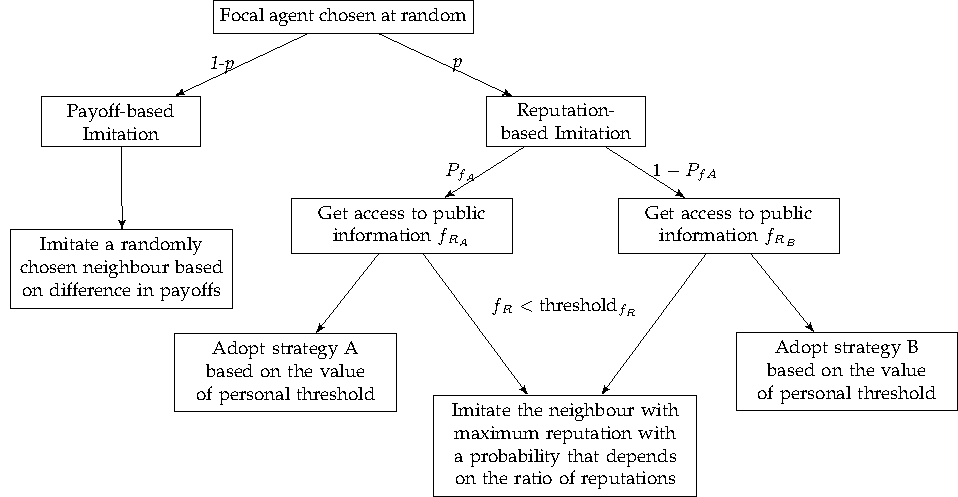
\includegraphics[keepaspectratio=true,scale=0.6]{opflow}}
 \makebox[\linewidth]{%        to center the image
 		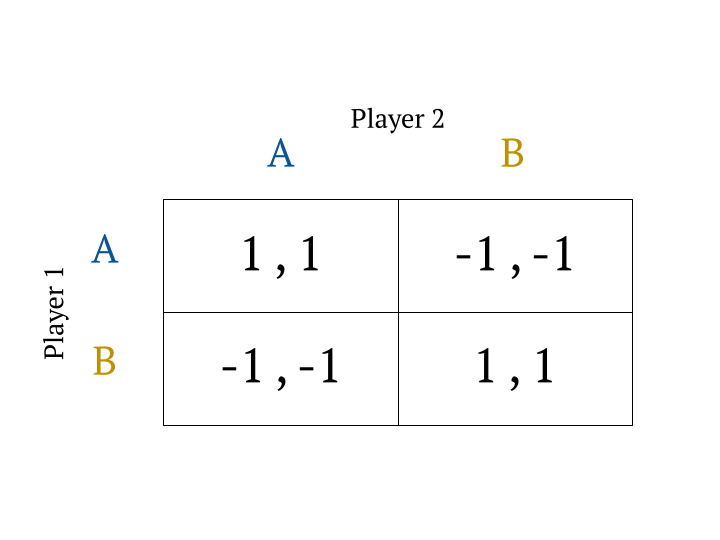
\includegraphics[keepaspectratio=true,scale=0.2]{graphs/payoff-matrix-op}}
 	\vspace{-1cm}
 	\captionof{figure}{\footnotesize Flowchart and payoff matrix for the opinion dynamics model. An agent gets positive payoff for interactions with same strategy neighbours. This may lead to formation of clusters. }\label{flow:opdyn}%      only if needed  
 \end{minipage}

% Results for opdyn
\begin{figure}[h]
	\centering
	\begin{subfigure}[b]{0.4\textwidth}
		\centering
		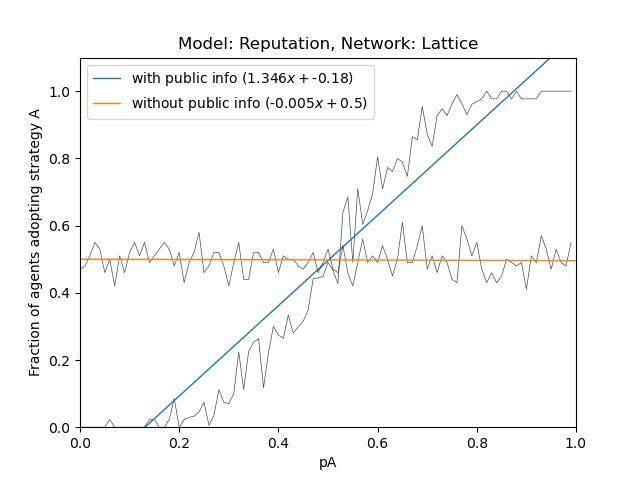
\includegraphics[width=\textwidth]{graphs/lat-pAvsnormal}
		\caption{}
		\label{fig:lat-pA}
	\end{subfigure}
	\begin{subfigure}[b]{0.4\textwidth}
		\centering
		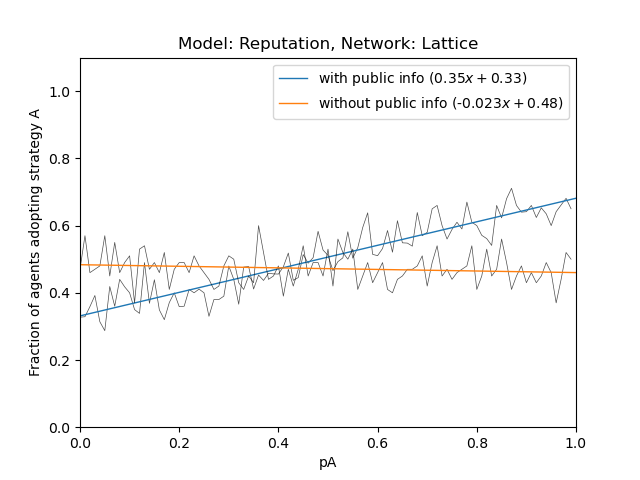
\includegraphics[width=\textwidth]{graphs/sf-pAvsnormal}
		\caption{}
		\label{fig:sf-pA}
	\end{subfigure}
	\caption{\footnotesize \textit{(a)} Network: Lattice. Low values of $ P_{A} $ means that public information (\fr) related to strategy B is more likely to be used by the agents. High values of $ P_{A} $ show a very significant increase in the fraction of population adopting strategy A. \textit{(b)} Network: Scalefree. }
	\label{fig:opdyn}
\end{figure}

 \section{Conclusion} \label{sec:conclusion}
 In this project, three new models that promote the emergence and persistence of cooperation in a structured population were explored. The effect of reputation as a social reward mechanism and public information as a trust mechanism on networked populations was observed. There was a significant increase in the equilibrium values of $ f_{C} $ in all the models. We applied one of the models (\textit{Rep}) to a real-world situation. It was observed that increase in popularity of an opinion and its effective dissemination among the agents increases the fraction of agents that adopt that strategy (under equilibrium conditions). Further work on the topic can test how clusters are formed in the population and how the fraction of agents adopting a particular strategy would change with time. 
 
 
\appendix
 \section{Appendix} \label{appendix}
 \subsection{Model \textit{PDist}} \label{app:1}
 For the \textit{PDist} model, $ \Delta P$ varies as a function of the difference between the focal agent's payoff and the average nearest neighbor payoff, $p_\text{avg}$. The value of $ k_{pd} $ for all the simulations is taken to be $ 1.5 $.
 
 \begin{equation}\label{eq:deltap}
 	\Delta P = \Delta P_\text{max} \left[\frac{2}{1 + \exp[(p_{i} - p_{\text{avg}})/k_{pd}]} - 1\right]
 \end{equation}
 
 \subsection{Model \textit{fcT}}\label{app:2}
 When the focal agent does not have access to public information (\fc) then it has to use local information i.e. nearest neighbour payoffs. In equation \ref{eq:fcth}, $ a' $ is given by
 
 \begin{equation}
 	a' = 
 	\begin{cases}
 		\dfrac{a'_{\text{max}}}{1 + \exp[p_{i} - p_{\text{avg}}/k_{\fcm}]} & p_{i}>p_{\text{avg}} \\
 		0 & p_{i}\leq p_{\text{avg}}
 	\end{cases}
 \end{equation}

$ p_{\text{avg}} $ is the average nearest neighbour payoff. The value of $ a' $ and subsequently $ P_{t}^{s} $ is high if the difference in the focal agent's payoff and $ p_{\text{avg}} $ is high. For all the simulations, the parameter values are taken to be as follows: $ a'_{\text{max}} = 0.2$, $ k_{fc} = 1.5 $. 

 \begin{figure}[h]
	\centering
	\begin{subfigure}[b]{0.35\textwidth}
		\centering
		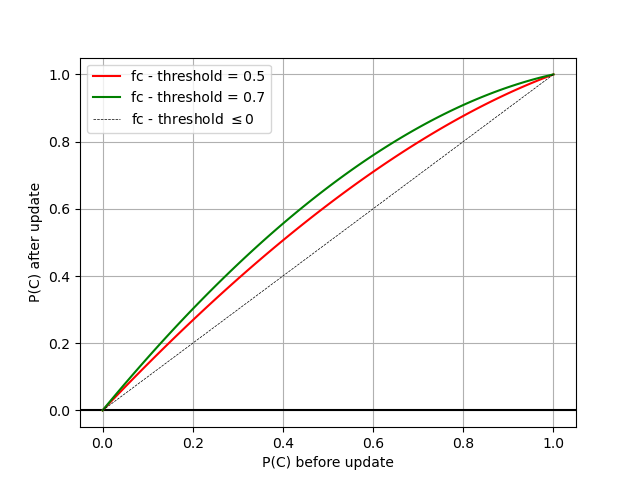
\includegraphics[width=\textwidth]{graphs/fc-threshold-probupdate}
		\caption{}
		\label{fig:fct1}
	\end{subfigure}
	\begin{subfigure}[b]{0.23\textwidth}
		\centering
		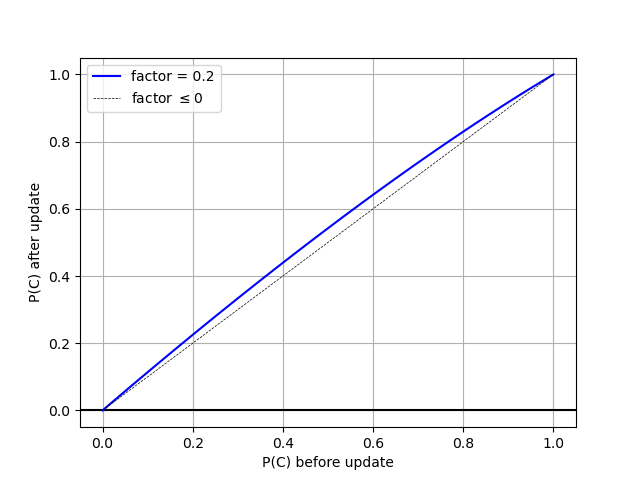
\includegraphics[width=\textwidth]{graphs/fc-threshold-probupdate-2}
		\caption{}
		\label{fig:fct2}
	\end{subfigure}
\begin{subfigure}[b]{0.23\textwidth}
	\centering
	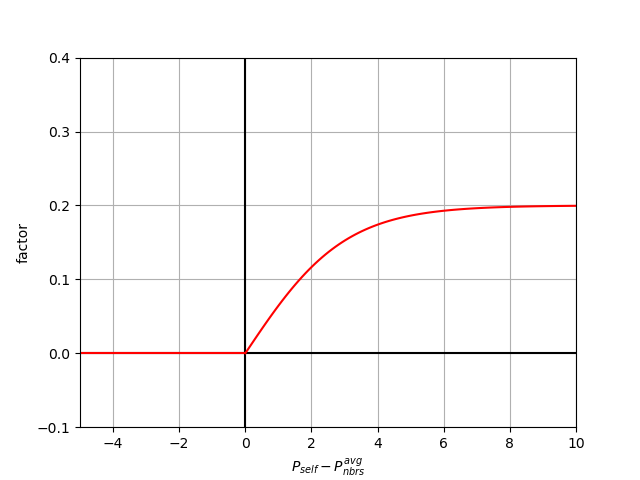
\includegraphics[width=\textwidth]{graphs/fc-threshold-probupdate-factor}
	\caption{}
	\label{fig:fct3}
\end{subfigure}
	\caption{\footnotesize \textit{(a)} Shows $ P_{t}^{C}  $ before and after updation. The curves are for different values of (\fc $ - \text{threshold}_{\fcm} $). \textit{(b)} show how $ P_{t}^{C}  $ evolves in the absence of public information. \textit{(c)} is the variation of factor $ a' $ with the difference in payoffs. }
	\label{fig:fct}
\end{figure}

\subsection{Model \textit{Rep}}\label{app:3}
We use the usual Fermi-Dirac like probability function for this model. Updates based on public information take into account the reputation of the agent so that agents with a history of cooperation keep cooperating in the future. Updates based on local information take into account the difference in reputation as agents are likely to be influenced by their nearest neighbours, especially by those who have a higher reputation. \par 
Every time an agent chooses to cooperate, its reputation is increased. Reputation before and after increase are denoted by $ \text{rep}_{i} $ and $ \text{rep}_{f} $. 

\begin{equation}
	\text{rep}_{f} = \text{rep}_{i}(2-  \text{rep}_{i} )  
\end{equation}

For all the simulations, the parameter values are taken to be as follows: $ k_{r_{1}} = 0.25$, $ k_{r_{2}} = 0.05 $, $ k = 0.1  $ (for payoff-based imitation). 

\begin{figure}[h]
		\centering
		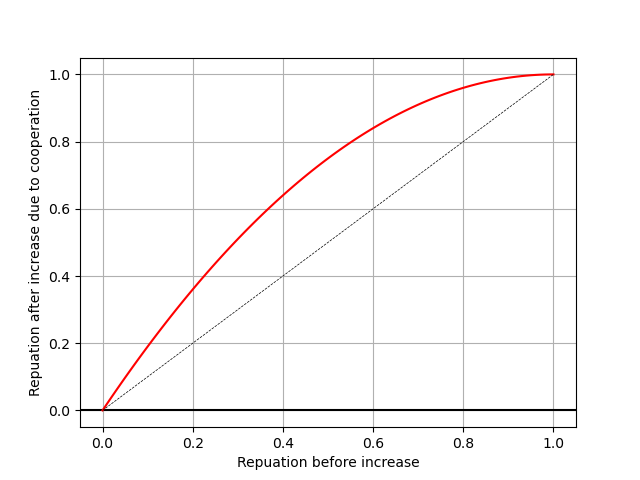
\includegraphics[width=0.4\textwidth]{graphs/reputation_inc}
	\caption{\footnotesize The graph shows the value of reputation before and after updation. It starts at 0 and tapers off near 1. The initial reputation for all agents is set to be 0.05 }
	\label{fig:repinc}
\end{figure}

 \subsection{Opinion Dynamics Model (Futher Details)}\label{app:4}
 The transition probability function for imitation based on reputation is given by equation \ref{eq:optrfn}.  
\par  

 \begin{equation} \label{eq:optrfn}
 	W(s_{i} \leftarrow s_{j}) = 
 	\begin{cases}
 		\dfrac{1}{1 + \exp[\text{0.5-x}/k_{op_{1}}]} & x\geq 0\\
 		&\\
 		\dfrac{0.9}{1 + \exp[\text{x+5}/k_{op_{2}}]} & x<0
 	\end{cases}
 \end{equation}

We choose this particular functional form because it satisfies the following conditions - 
\begin{enumerate}
	\item Reaches maximum at $ +1 $: this is so that any agent that encounters another agent with similar reputation will imitate it with a high probability.
	\item Value at $ -1 $ is very low: this is so that the probability of imitating an agent with reputation equal in magnitude but opposite in sign is negligible
	\item Probability is high for large negative values: this is to model the influence of high-reputation agents on low reputation individuals with an opposite sign
\end{enumerate}

\begin{figure}[h]
	\centering
	\begin{subfigure}[b]{0.5\textwidth}
		\centering
		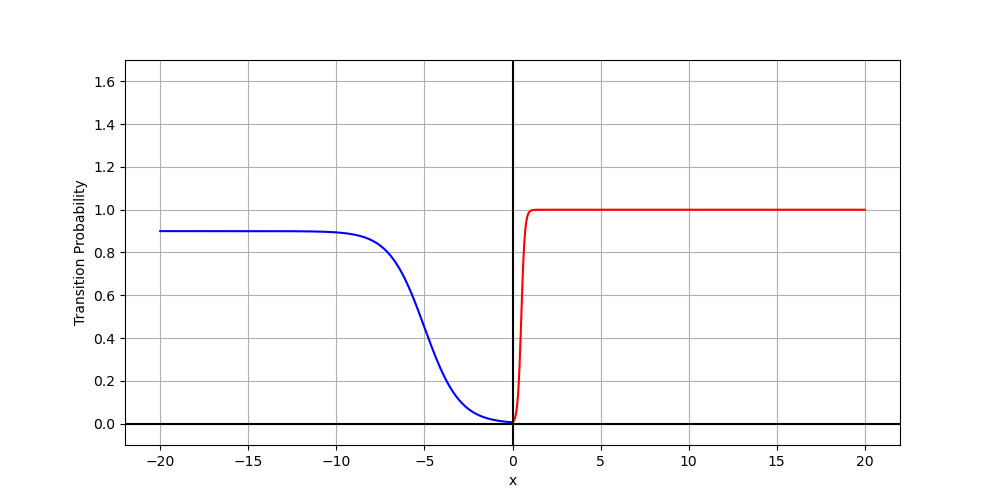
\includegraphics[width=\textwidth]{graphs/transprob_opdyn}
		\caption{}
		\label{fig:oprep1}
	\end{subfigure}
	\begin{subfigure}[b]{0.3\textwidth}
		\centering
		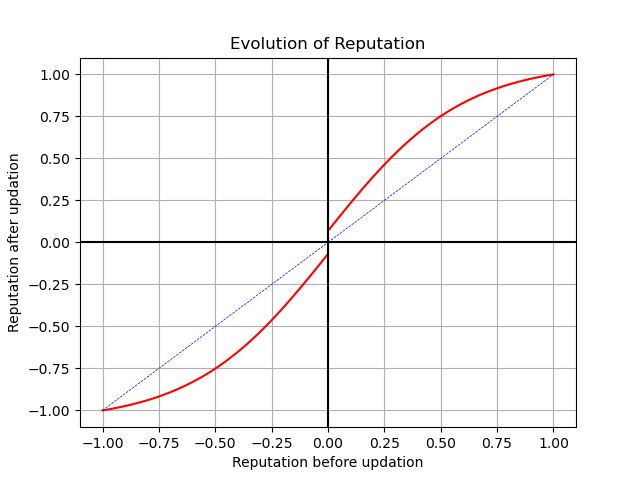
\includegraphics[width=\textwidth]{graphs/repevol_C3}
		\caption{}
		\label{fig:oprep2}
	\end{subfigure}
	\caption{\footnotesize \textit{(a)} is the transition probability function for reputation based imitation. We can see that it follows the 3 conditions listed. \textit{(b)} shows how the reputation of an agent evolves. Reputation goes in only one direction (either positive or negative). }
	\label{fig:oprep}
\end{figure}

If the updation of strategy is based in public information (i.e. if \fr{} is greater than the personal threshold), then the probability of adopting a given strategy is given by equation \ref{eq:optrfn2}. 

\begin{equation} \label{eq:optrfn2}
	\begin{split}
		&P_{t}^{s} = 	\frac{1}{1 + \exp[-\text{threshold}_{\frm}/k_{op_{3}}]} \\
		&P_{t}^{-s} = 1- P_{t}^{s}
	\end{split}
\end{equation}

In the above equation, $ s $ is A if the focal agent's reputation is positive and B if it is negative. For all the simulations, the parameter values are taken to be as follows: $ k_{op_{1}} = 0.1$, $ k_{op_{2}} = 1 $, $ k_{op_{3}} = 0.25 $.

\bibliographystyle{unsrt}
\bibliography{references}

\end{document}